\renewcommand{\theequation}{\theenumi}
\begin{enumerate}[label=\arabic*.,ref=\thesubsection.\theenumi]
\numberwithin{equation}{enumi}
\item
Let
\begin{equation}
\mathbf{y} = \mathbf{s}+ \mathbf{n}
\end{equation}
where $\mathbf{s} \in \cbrak{\mathbf{s}_0,\mathbf{s}_1,\mathbf{s}_2, \mathbf{s}_3}$ and
\begin{align}
\mathbf{s}_0 &= 
\begin{pmatrix*}
\sqrt{E_s}\\
0
\end{pmatrix*},
\mathbf{s}_1 = 
\begin{pmatrix*}
0\\
\sqrt{E_s}
\end{pmatrix*},
\\
\mathbf{s}_2 &= 
\begin{pmatrix*}
-\sqrt{E_s}\\
0
\end{pmatrix*},
\mathbf{s}_3 = 
\begin{pmatrix*}
0\\
-\sqrt{E_s}
\end{pmatrix*},
\\
E\sbrak{\mathbf{n}} &= \mathbf{0}, E\sbrak{\mathbf{n}\mathbf{n}^T} = \sigma^2 \mathbf{I}
\end{align}
%
\item Show that the MAP decision for detecting $\mathbf{s}_0$ results in
\begin{equation}
\abs{y_2} < y_1
\end{equation}

\item Express $\pr{\hat{\mathbf{s}} = \mathbf{s}_0|\mathbf{s} = \mathbf{s}_0}$ in terms of $r_1, r_2$.
Let $X=n_2-n_1, Y = -n_2-n_1$, where $\mathbf{n}=\brak{n_1,n_2}$.
Their correlation coefficient is defined as
%
\begin{align}
\rho = \frac{E\sbrak{\brak{X-\mu_x}\brak{Y-\mu_y}}}{\sigma_x\sigma_y}
\end{align}
%
$X$ and $Y$ are said to be uncorrelated if $\rho = 0$

\item
Show that  $X$ and $Y$ are uncorrelated. 
Verify this numerically.

\item
Show that $X$ and $Y$ are independent, i.e. $p_{XY}(x,y) = p_{X}(x)p_{Y}(y)$.

\item
Show that $X,Y \sim \mathcal{N}\brak{0,N_0}$.

\item
Show that 
\begin{equation}
\pr{\hat{\mathbf{s}} = \mathbf{s}_0|\mathbf{s} = \mathbf{s}_0} =\pr{ X < \sqrt{E_s},  Y < \sqrt{E_s}}.
\end{equation}

\item
Show that 
\begin{equation}
\pr{ X < \sqrt{E_s},  Y < \sqrt{E_s}} = \brak{1-\qfunc{\sqrt{\frac{E_s}{N_0}}}}^2
\end{equation}

\item
Verify the above through simulation.

\solution 
This is shown in Fig. \ref{fig:qpsk} through the following code.
\begin{lstlisting}
codes/modulation/qpsk.py
\end{lstlisting}
%
\begin{figure}[!h]
\centering
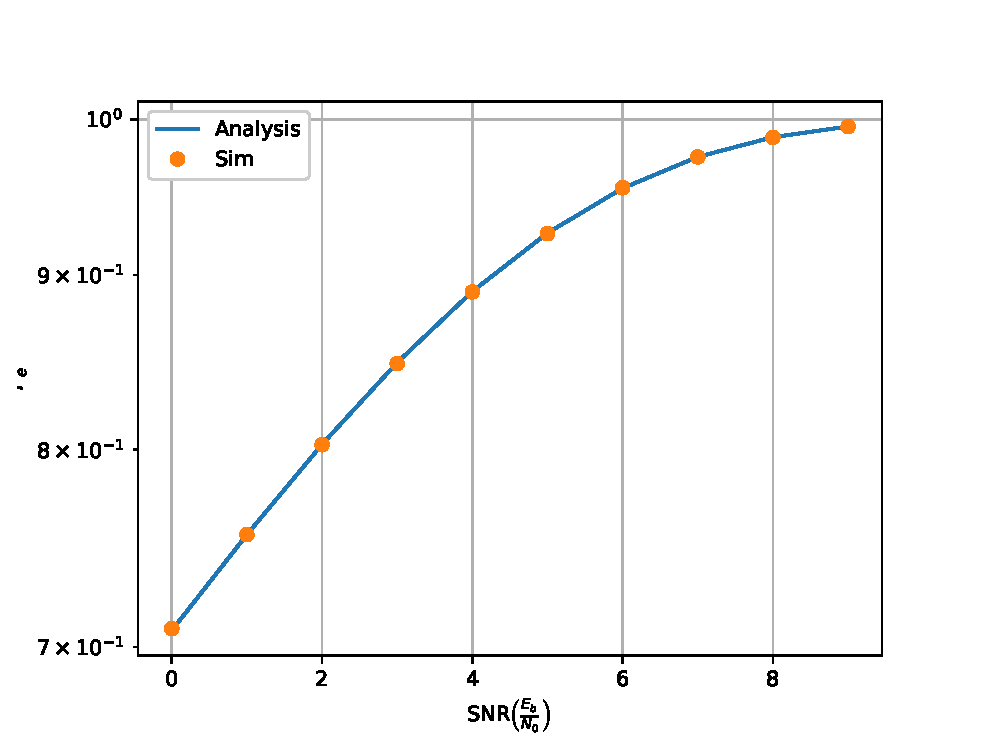
\includegraphics[width=\columnwidth]{./modulation/manual/figs/qpsk.eps}
\caption{}
\label{fig:qpsk}
\end{figure}
\item
Modify the above script to obtain the probability of symbol error.


%\begin{enumerate}
%\item 
%\item 
%\item 
%\item 
%\item 
%\item 
%\\
%\solution Given we transmitted $s_0$, the probability of decoding it as $s_0$ is given by 
%\begin{equation}
%\pr{\hat{\mathbf{s}} = \mathbf{s}_0|\mathbf{s} = \mathbf{s}_0} = \pr{-n_2<\sqrt{E_s}+n_1,\sqrt{E_s}+n_1>n_2} 
%\end{equation}
%\begin{equation}
%\implies \pr{\hat{\mathbf{s}} = \mathbf{s}_0|\mathbf{s} = \mathbf{s}_0} = \pr{X<\sqrt{E_s},Y<\sqrt{E_s}}
%\end{equation}
%\\
%Where, $X=n_2-n_1, Y=-n_2-n_1$. Also $X,Y \sim \mathcal{N}\brak{0,2\sigma^2}$ and are independent. 
%\item Show that 
%\begin{equation}
%\pr{ X < \sqrt{E_s},  Y < \sqrt{E_s}} = \brak{1-\qfunc{\sqrt{\frac{E_s}{N_0}}}}^2
%\end{equation}
%\solution 
%\begin{equation}
%\pr{X < A, Y < A} = \pr{X < A}\pr{Y < A}
%\end{equation}
%\begin{equation}
%\implies \pr{X < A, Y < A} = \brak{1-\qfunc{\frac{A}{\sqrt{2}\sigma}}}^2
%\end{equation}
%\item 
%\\
%
%\item 
\end{enumerate}
%
